\documentclass[aspectratio=169,12pt]{beamer}

\usepackage[utf8]{inputenc}
\usepackage[T5]{fontenc}
\usepackage{mathptmx}
\usepackage[vietnamese]{babel}
\usepackage{amsmath,amssymb,amsfonts,bm}
\usepackage{graphicx}
\usepackage{booktabs}
\usepackage{array}
\usepackage{multicol}
\usepackage[table]{xcolor}
\usepackage{tikz}
\usetikzlibrary{calc}
\usepackage{tcolorbox}

\usetheme{Madrid}
\usefonttheme{serif}
\usecolortheme{default}
\setbeamertemplate{navigation symbols}{}
\setbeamertemplate{footline}[frame number]

\definecolor{hcmutblue}{RGB}{0,76,153}
\definecolor{hcmutlight}{RGB}{232,242,252}
\setbeamercolor{structure}{fg=hcmutblue}
\setbeamercolor{frametitle}{bg=hcmutlight,fg=hcmutblue}
\setbeamercolor{title}{fg=hcmutblue}

\title{Đạo hàm riêng của hàm nhiều biến\\và ứng dụng của nó}
\subtitle{Slide thuyết trình dựa trên báo cáo môn Giải tích 2 (MT1005)}
\author{Nhóm 01}
\institute{Trường Đại học Bách khoa -- ĐHQG TP.HCM\\Khoa Khoa học Ứng dụng}
\date{Tháng 4 năm 2026}

\newcommand{\divideritem}[3]{%
  \ifnum#1=#2
    \def\itemfill{hcmutblue}%
    \def\itemtext{hcmutblue}%
  \else
    \def\itemfill{gray!25}%
    \def\itemtext{gray!45}%
  \fi
  \noindent
  \tikz[baseline=-0.6ex]\node[circle,fill=\itemfill,text=white,minimum size=2.1em,inner sep=0pt,font=\bfseries\small]{#1};%
  \hspace{0.6em}{\color{\itemtext}\Large #3}\par\vspace{0.45cm}%
}

\newcommand{\sectiondivider}[1]{%
\begin{frame}[plain]
\vspace{0.35cm}
\divideritem{1}{#1}{Mở đầu}
\divideritem{2}{#1}{Công nghệ sử dụng}
\divideritem{3}{#1}{Kiến trúc hệ thống}
\divideritem{4}{#1}{Thiết kế chức năng \& giao diện}
\divideritem{5}{#1}{Kiểm định chất lượng}
\divideritem{6}{#1}{Tổng kết}
\end{frame}
}

\begin{document}

\begin{frame}[plain]
  \centering

  \vspace{0.1cm}
  \begin{minipage}[c]{0.10\textwidth}
      \centering
      
\includegraphics[width=0.82\linewidth]{image/HCMUT_official_logo.png}
  \end{minipage}
  \hspace{0.01\textwidth}
  \begin{minipage}[c]{0.76\textwidth}
      \centering
      {\normalsize \textbf{Trường Đại học Bách khoa -- ĐHQG TP.HCM}}\\[1pt]
      {\normalsize \textbf{Khoa Khoa học và Kỹ thuật Máy tính}}
  \end{minipage}

  \vspace{0.35cm}

  {\small \textbf{BÁO CÁO KẾT QUẢ TRAINING}}\\[3pt]
  {\footnotesize \textbf{Chương trình đào tạo IVS $\times$ RD--SEAI: Software Project Lifecycle}}

  \vspace{0.45cm}

  {\Large \textbf{XÂY DỰNG HỆ THỐNG ỨNG TUYỂN VIỆC LÀM}}

  \vspace{0.45cm}

  {\large \textbf{Nhóm 02}}\\[6pt]
  {\normalsize \textbf{Hướng dẫn:} Công ty IVS}

  \vfill
  {\small Thành phố Hồ Chí Minh, tháng 5 năm 2026}
\end{frame}

\begin{frame}{Danh sách thành viên}
  \centering
  \footnotesize
  \renewcommand{\arraystretch}{1.35}
  \rowcolors{2}{gray!10}{white}

  \begin{tabular}{c c p{0.26\textwidth} p{0.42\textwidth}}
    \toprule
    \rowcolor{blue!20}
    \textbf{STT} & \textbf{MSSV} & \centering\arraybackslash\textbf{Họ và tên} & \centering\arraybackslash\textbf{Email} \\
    \midrule
    1 & 2211322 & Đoàn Trí Hùng & \ttfamily\scriptsize hung.doantrymybest@hcmut.edu.vn \\
    2 & 2211190 & Lê Huỳnh Huy & \ttfamily\scriptsize huy.lehuynh2004@hcmut.edu.vn \\
    3 & 2211562 & Vương Quang Khải & \ttfamily\scriptsize khai.vuongquang@hcmut.edu.vn \\
    4 & 2211670 & Bùi Minh Khôi & \ttfamily\scriptsize khoi.buibachkhoa22@hcmut.edu.vn \\
    5 & 2252377 & Nguyễn Minh Khôi & \ttfamily\scriptsize khoi.nguyenminhcs22@hcmut.edu.vn \\
    6 & 2213772 & Lê Đức Anh Tuấn & \ttfamily\scriptsize tuan.leqn04@hcmut.edu.vn \\
    7 & 2212331 & Trương Minh Nguyên & \ttfamily\scriptsize nguyen.truongpythonai@hcmut.edu.vn \\
    8 & 2212922 & Nguyễn Quang Sáng & \ttfamily\scriptsize sang.nguyennqs@hcmut.edu.vn \\
    \bottomrule
  \end{tabular}
\end{frame}

\begin{frame}{Nội dung trình bày}
  \small
  \tableofcontents
\end{frame}

\section{Giới thiệu đề tài}
\sectiondivider{1}
\begin{frame}{Bối cảnh \& vấn đề}
  \begin{itemize}
    \item Thị trường lao động số: khối lượng hồ sơ và vị trí tuyển lớn, cập nhật nhanh.
    \item Quản lý thủ công (email, Excel, giấy tờ) \textbf{không đủ} quy mô và tốc độ tuyển dụng hiện đại.
    \item Cần \textbf{một nền tảng thống nhất} để theo dõi ứng viên từ đăng tin đến quyết định.
  \end{itemize}
\end{frame}

\begin{frame}{ATS là gì?}
  \begin{block}{Định nghĩa}
    \textbf{ATS (Applicant Tracking System)} --- phần mềm số hóa và tự động hóa quy trình tuyển dụng:
    đăng tin, tiếp nhận hồ sơ, sàng lọc, lịch phỏng vấn, đánh giá, ra quyết định.
  \end{block}
  \vspace{0.3cm}
  \begin{itemize}
    \item Dự án trong khuôn khổ \textbf{IVS $\times$ RD--SEAI: Software Project Lifecycle}.
    \item Nhóm trải nghiệm trọn vòng đời phát triển phần mềm thực tế.
  \end{itemize}
\end{frame}

\begin{frame}{Hai thành phần chính của hệ thống}
  \begin{columns}[T]
    \column{0.48\textwidth}
    \begin{block}{Job Portal (công khai)}
      \small
      \begin{itemize}
        \item Tìm kiếm, xem chi tiết việc làm
        \item Nộp đơn ứng tuyển
        \item Tối ưu SEO, thân thiện người dùng
      \end{itemize}
    \end{block}
    \column{0.48\textwidth}
    \begin{block}{Dashboard nội bộ}
      \small
      \begin{itemize}
        \item HR, Admin, Interviewer
        \item Pipeline tuyển dụng, KPI
        \item Quản lý tin, đơn, phỏng vấn
      \end{itemize}
    \end{block}
  \end{columns}
\end{frame}

\begin{frame}{Mục tiêu theo đối tượng}
  \small
  \begin{itemize}
    \item \textbf{Ứng viên:} tìm việc, quản lý hồ sơ, nộp đơn, theo dõi trạng thái minh bạch.
    \item \textbf{HR / Admin:} tin đa kênh, pipeline Kanban, báo cáo hiệu suất.
    \item \textbf{Interviewer:} lịch PV, hồ sơ ứng viên, scorecard, cập nhật kết quả.
    \item \textbf{Đội phát triển:} chuẩn kỹ thuật hiện đại, bảo mật, mở rộng và bảo trì.
  \end{itemize}
\end{frame}

\begin{frame}{Phạm vi: bảy module chức năng (A--G)}
  \footnotesize
  \begin{enumerate}
    \item \textbf{A -- Public \& Landing:} trang chủ, danh sách/chi tiết job, nộp đơn.
    \item \textbf{B -- Authentication:} đăng nhập, đăng ký, OTP, quên/đổi mật khẩu.
    \item \textbf{C -- Candidate:} dashboard ứng viên, hồ sơ, đơn, lịch PV.
    \item \textbf{D -- Dashboard nội bộ:} KPI, báo cáo, quản trị người dùng.
    \item \textbf{E -- Applications:} pipeline đơn, trạng thái, lịch sử thay đổi.
    \item \textbf{F -- Interviews:} lịch PV, đánh giá ứng viên.
    \item \textbf{G -- Jobs:} tạo/sửa tin, đa kênh đăng tuyển.
  \end{enumerate}
\end{frame}

\begin{frame}{Quy mô triển khai (theo báo cáo)}
  \begin{itemize}
    \item Khoảng \textbf{22 màn hình} và \textbf{hơn 30 API} REST (envelope JSON thống nhất).
    \item Tài liệu \textbf{Detail Design} theo từng module; bộ \textbf{UTC / UTE / ITC / ITE}.
    \item Phân quyền \textbf{RBAC bốn role} vận hành ổn định trên toàn route.
  \end{itemize}
\end{frame}

\begin{frame}{Phân công nhóm (trụ cột thiết kế)}
  \small
  \begin{itemize}
    \item \textbf{Nhóm trưởng:} Đoàn Trí Hùng --- điều phối, quy ước Git, báo cáo tiến độ.
    \item \textbf{Module -- chủ điểm:} Khải (A), Huy (B), Sáng (C), Khôi D. (D), Tuấn (E), Khôi B. (F), Hùng \& Nguyên (G).
  \end{itemize}
  \vspace{0.35cm}
  {\footnotesize Mỗi thành viên phụ trách phân hệ từ thiết kế đến triển khai theo báo cáo chi tiết.}
\end{frame}

\section{Công nghệ sử dụng}
\sectiondivider{2}
\begin{frame}{Stack công nghệ (tóm tắt)}
  \small
  \begin{itemize}
    \item \textbf{Framework:} Next.js~16 (App Router), TypeScript strict.
    \item \textbf{UI:} Tailwind CSS~4, shadcn/ui (Radix), TanStack Query~v5.
    \item \textbf{Dữ liệu:} MariaDB, Prisma~7 (adapter MariaDB), REST Route Handlers.
    \item \textbf{Bảo mật:} JWT (jose, HS256), cookie \texttt{httpOnly}, bcrypt 12 rounds.
    \item \textbf{Tích hợp:} Appwrite Storage (CV), Resend (email), Zod validation.
  \end{itemize}
\end{frame}

\begin{frame}{Next.js}
  \begin{center}
    
\includegraphics[width=0.72\textwidth,height=3.6cm,keepaspectratio]{image/technology/nextjs.jpeg}
  \end{center}
  \vspace{-0.2cm}
  {\small \textit{Full-stack React: Server/Client Components, Route Handlers, metadata SEO.}}
\end{frame}

\begin{frame}{Prisma ORM}
  \begin{center}
    
\includegraphics[width=0.62\textwidth,height=3.4cm,keepaspectratio]{image/technology/prisma.png}
  \end{center}
  \vspace{-0.2cm}
  {\small \textit{Schema-first, migrations, truy vấn kiểu an toàn với MariaDB.}}
\end{frame}

\begin{frame}{TanStack Query}
  \begin{center}
    
\includegraphics[width=0.72\textwidth,height=3.5cm,keepaspectratio]{image/technology/tanstack.png}
  \end{center}
  \vspace{-0.2cm}
  {\small \textit{Cache, refetch và trạng thái tải dữ liệu REST phía client.}}
\end{frame}

\begin{frame}{shadcn/ui}
  \begin{center}
    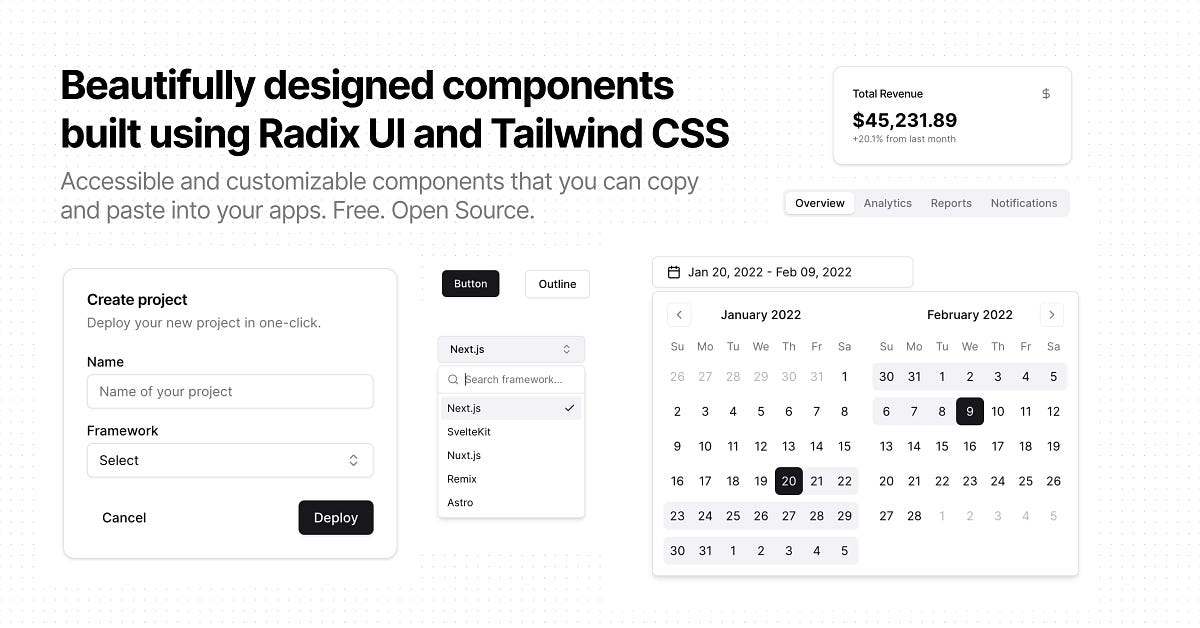
\includegraphics[width=0.62\textwidth,height=3.2cm,keepaspectratio]{image/technology/shadcnui.jpg}
  \end{center}
  \vspace{-0.2cm}
  {\small \textit{Component tái sử dụng trên Radix UI + Tailwind; dark mode.}}
\end{frame}

\section{Kiến trúc hệ thống}
\sectiondivider{3}
\begin{frame}{Kiến trúc tổng quan}
  \small
  \begin{itemize}
    \item \textbf{Client:} React~19, Tailwind \& shadcn/ui, TanStack Query đồng bộ REST.
    \item \textbf{Next.js (cùng repo):} \texttt{app/*} UI; \texttt{app/api/**/*} REST; \texttt{middleware.ts} RBAC sớm.
    \item \textbf{Persistence:} Prisma~7 + MariaDB --- giao dịch cho đơn \& metadata file.
    \item \textbf{Ngoài hệ:} Appwrite (blob CV), Resend (email giao dịch).
    \item \textbf{Phiên:} JWT trong cookie \texttt{httpOnly}, không lưu session DB.
  \end{itemize}
\end{frame}

\begin{frame}{Phân quyền RBAC (theo route)}
  \footnotesize
  \begin{tabular}{@{}p{0.36\textwidth}p{0.58\textwidth}@{}}
    \toprule
    \textbf{Vùng} & \textbf{Ai được truy cập?} \\
    \midrule
    \texttt{/}, \texttt{/jobs}, \texttt{/jobs/[slug]} & Mọi người (public) \\
    \texttt{/login}, \texttt{/register} & Khách (chưa đăng nhập) \\
    \texttt{/candidate} & Role \texttt{candidate} \\
    \texttt{/dashboard/*} & \texttt{admin}, \texttt{hr}, \texttt{interviewer} \\
    \bottomrule
  \end{tabular}
\end{frame}

\begin{frame}{Cấu trúc thư mục dự án (App Router)}
  \footnotesize
  \begin{itemize}
    \item \texttt{app/} --- trang \& API theo file-based routing (\texttt{(auth)/}, \texttt{jobs/}, \texttt{dashboard/}, \texttt{candidate/}, \texttt{api/}).
    \item \texttt{components/}, \texttt{hooks/}, \texttt{lib/} --- UI tái sử dụng, React Query, JWT, Zod.
    \item \texttt{prisma/} --- \texttt{schema.prisma}, migration, seed.
  \end{itemize}
\end{frame}

\section{Thiết kế chức năng \& giao diện}
\sectiondivider{4}
\begin{frame}{Module A -- Khu vực công khai}
  \begin{columns}[c]
    \column{0.42\textwidth}
    \small
    \begin{itemize}
      \item Trang chủ, danh sách job
      \item Chi tiết tin, modal nộp đơn
    \end{itemize}
    \column{0.56\textwidth}
    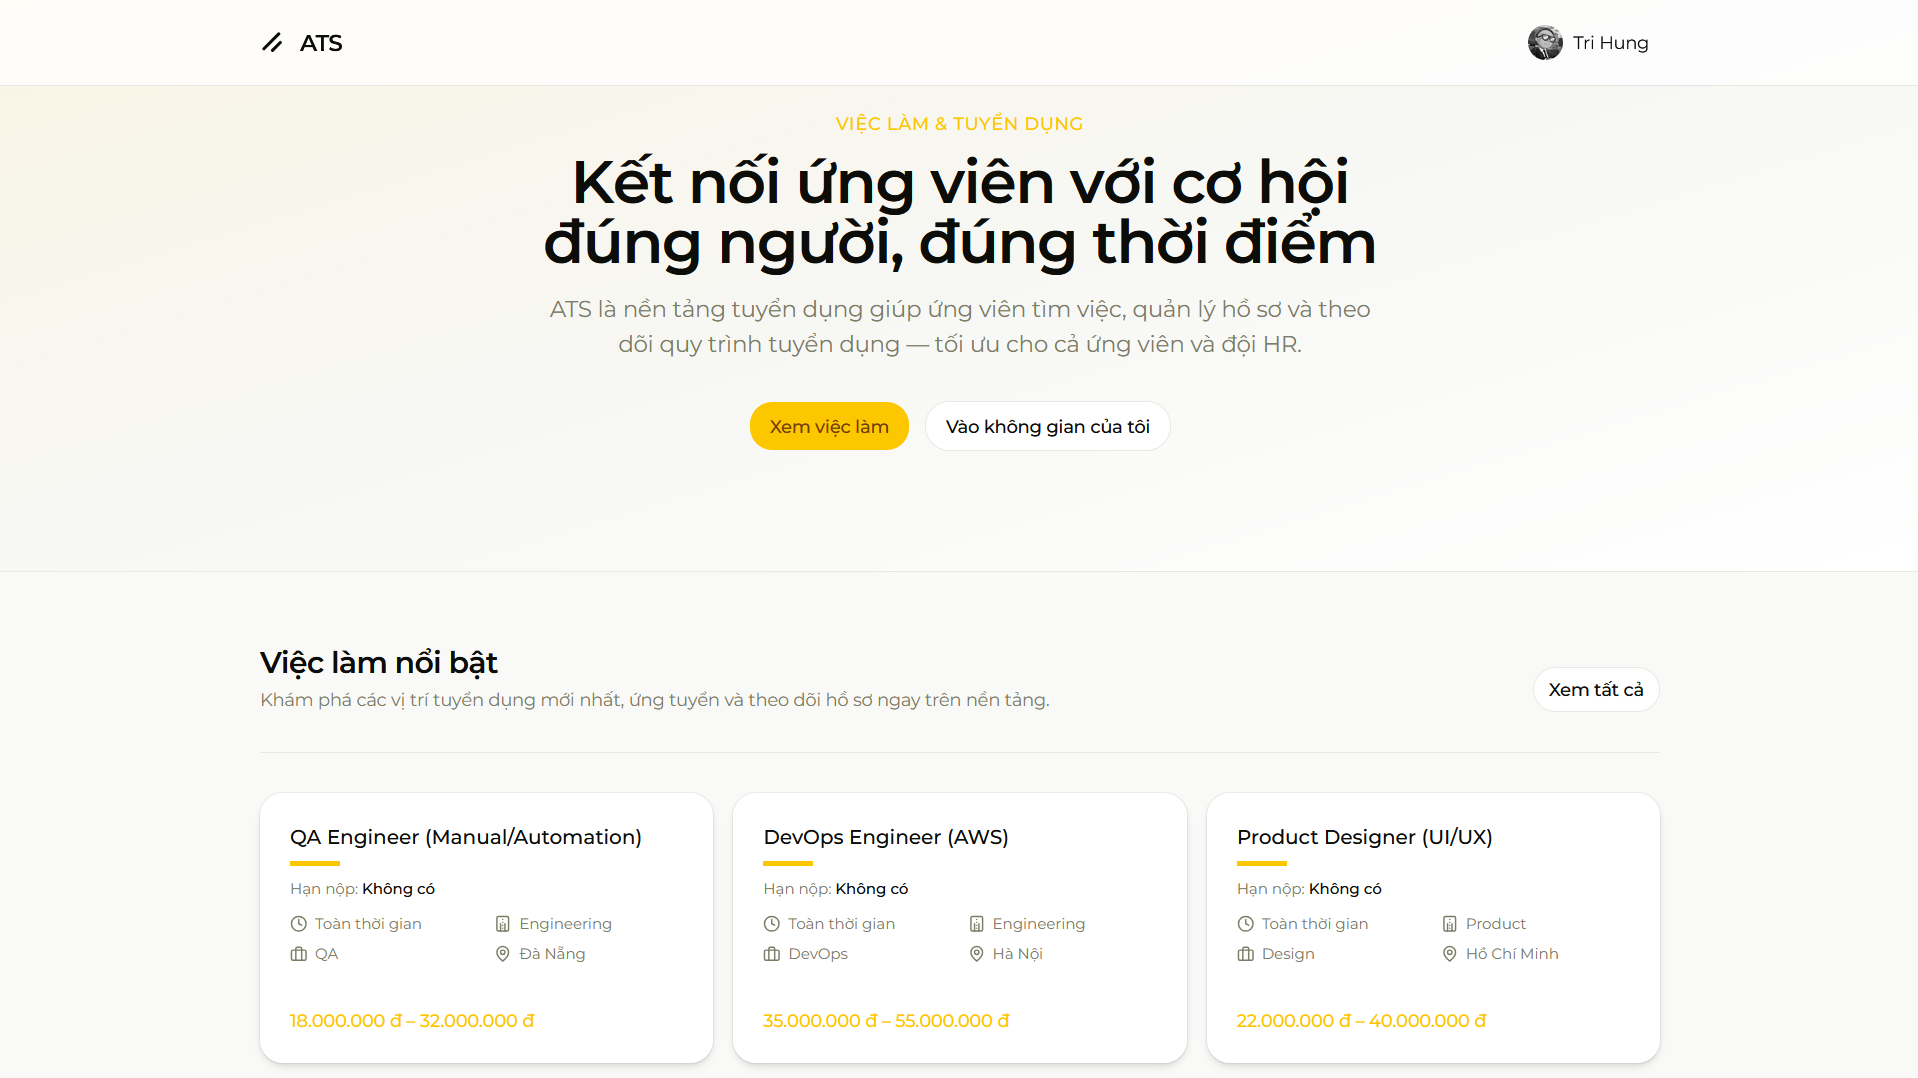
\includegraphics[width=\linewidth]{image/A/1.png}
  \end{columns}
\end{frame}

\begin{frame}{Module A -- Danh sách và chi tiết job}
  \begin{center}
    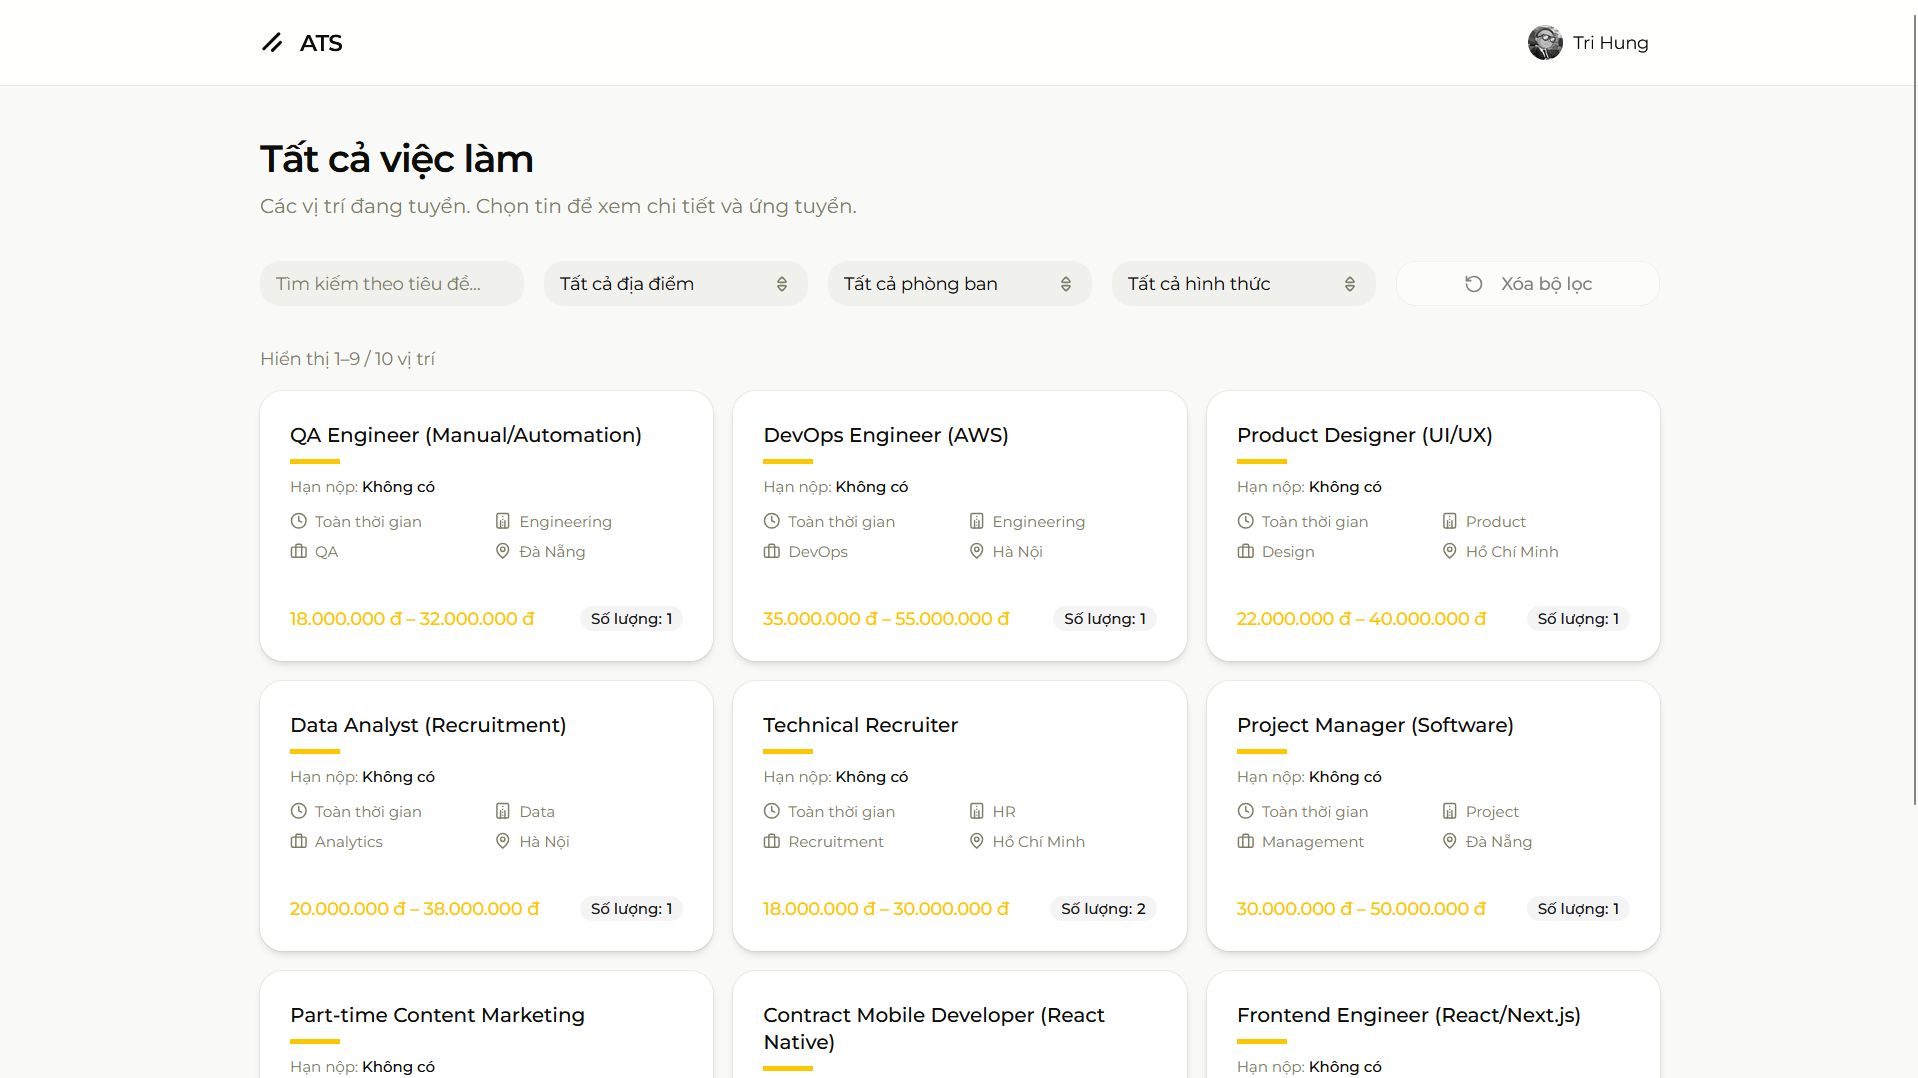
\includegraphics[width=0.46\textwidth]{image/A/2.png}\hfill
    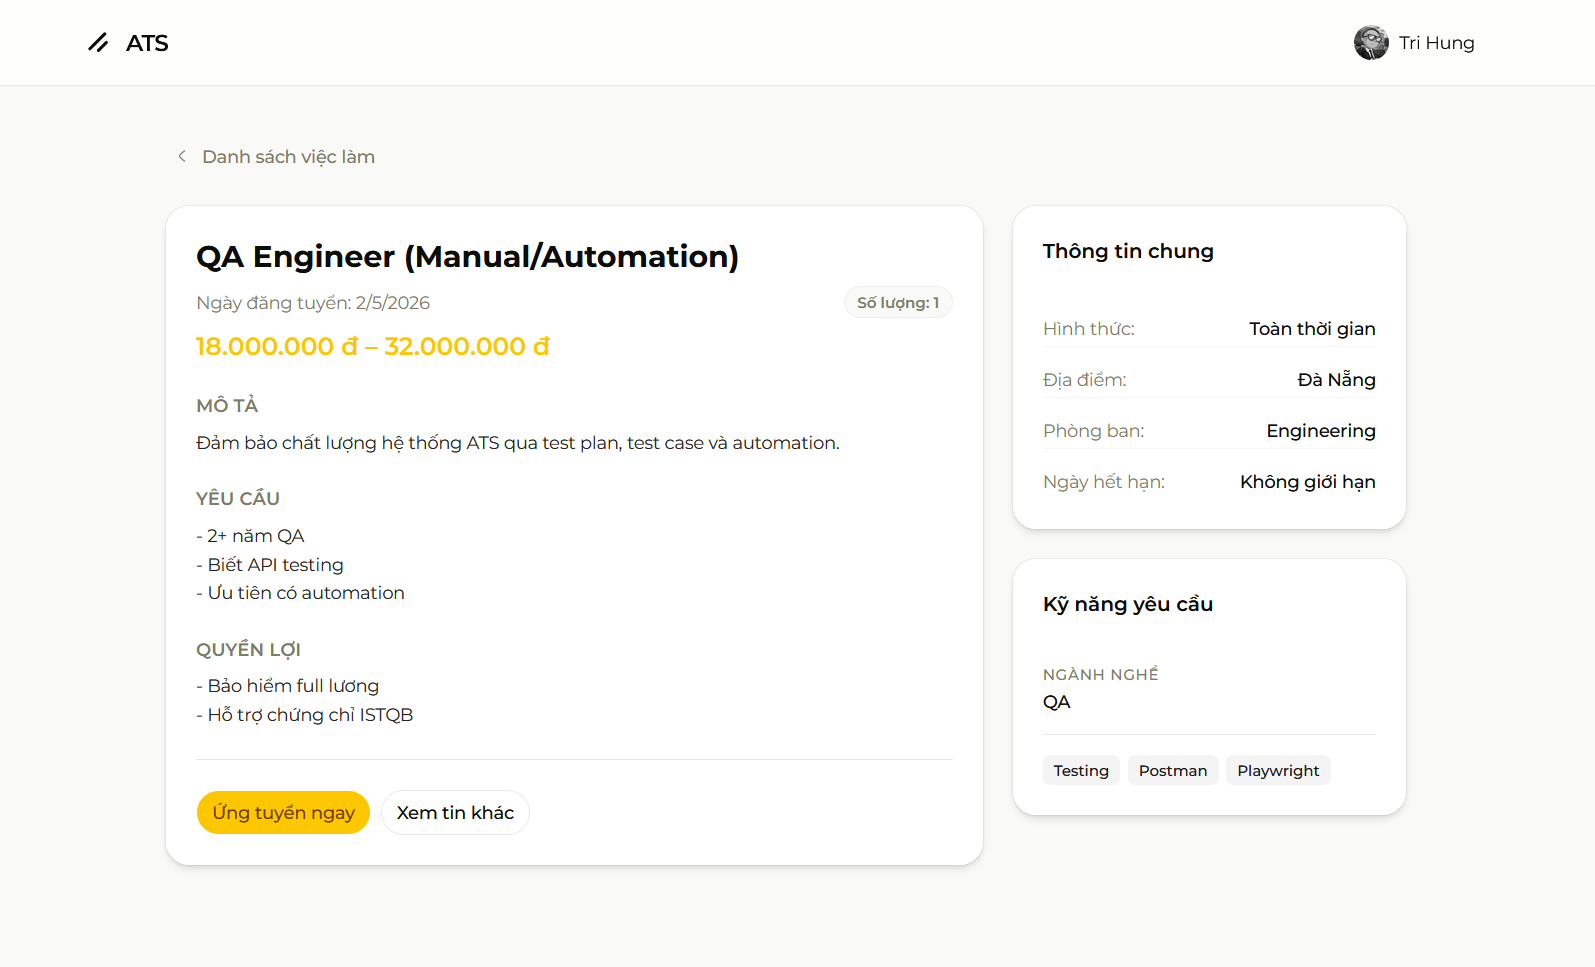
\includegraphics[width=0.46\textwidth]{image/A/3.png}
  \end{center}
\end{frame}

\begin{frame}{Module B -- Xác thực}
  \begin{columns}[c]
    \column{0.42\textwidth}
    \small Đăng nhập, đăng ký, OTP email, quên \& đổi mật khẩu.
    \column{0.56\textwidth}
    
\includegraphics[width=\linewidth]{image/B/1.png}
  \end{columns}
\end{frame}

\begin{frame}{Module C -- Khu vực ứng viên}
  \begin{columns}[c]
    \column{0.42\textwidth}
    \small Hồ sơ, đơn ứng tuyển, lịch phỏng vấn.
    \column{0.56\textwidth}
    
\includegraphics[width=\linewidth]{image/C/1.png}
  \end{columns}
\end{frame}

\begin{frame}{Module D -- Dashboard nội bộ}
  \begin{columns}[c]
    \column{0.42\textwidth}
    \small KPI, báo cáo, quản trị người dùng (role HR/Admin).
    \column{0.56\textwidth}
    
\includegraphics[width=\linewidth]{image/D/1.png}
  \end{columns}
\end{frame}

\begin{frame}{Module E -- Quản lý đơn ứng tuyển}
  \begin{columns}[c]
    \column{0.42\textwidth}
    \small Pipeline trạng thái, lịch sử thao tác (audit).
    \column{0.56\textwidth}
    
\includegraphics[width=\linewidth]{image/E/1.png}
  \end{columns}
\end{frame}

\begin{frame}{Module F -- Phỏng vấn}
  \begin{columns}[c]
    \column{0.42\textwidth}
    \small Lịch PV, đánh giá, scorecard.
    \column{0.56\textwidth}
    
\includegraphics[width=\linewidth]{image/F/1.png}
  \end{columns}
\end{frame}

\begin{frame}{Module G -- Quản lý tin tuyển dụng}
  \begin{columns}[c]
    \column{0.42\textwidth}
    \small Tạo/sửa job, trạng thái, đa kênh đăng tin.
    \column{0.56\textwidth}
    
\includegraphics[width=\linewidth]{image/G/1.png}
  \end{columns}
\end{frame}

\section{Kiểm định chất lượng}
\sectiondivider{5}
\begin{frame}{Chiến lược kiểm thử}
  \small
  \begin{itemize}
    \item \textbf{Unit / API:} endpoint độc lập --- thành công, lỗi validation, lỗi auth.
    \item \textbf{Integration:} luồng E2E (đăng ký $\rightarrow$ OTP $\rightarrow$ đăng nhập $\rightarrow$ nộp đơn\dots).
    \item \textbf{Manual:} kịch bản UI theo UTC và màn hình Detail Design.
  \end{itemize}
  \vspace{0.35cm}
  {\footnotesize Bộ chứng cứ: UTE, ITC, ITE theo tài liệu nhóm (báo cáo mục Kiểm định).}
\end{frame}

\begin{frame}{Ví dụ phạm vi test (Module A \& ITC)}
  \footnotesize
  \begin{itemize}
    \item \textbf{Public:} xem trang chủ, tìm kiếm/lọc job, chi tiết, nộp đơn (có/không đăng nhập).
    \item \textbf{ITC:} luồng đăng ký--xác minh--đăng nhập; tuyển dụng đầy đủ; phỏng vấn; quên mật khẩu.
  \end{itemize}
\end{frame}

\section{Tổng kết}
\sectiondivider{6}
\begin{frame}{Kết quả đạt được}
  \small
  \begin{itemize}
    \item \textbf{Kỹ thuật:} Next.js~16 + Prisma~7 + MariaDB; JWT tự triển khai; API REST envelope thống nhất; TypeScript end-to-end.
    \item \textbf{Nghiệp vụ:} 7 module (A--G), hơn 30 API, tài liệu Detail Design \& test cases đi kèm.
    \item \textbf{Quy trình:} Git nhánh tính năng, phân công theo module, tài liệu hóa đầy đủ.
  \end{itemize}
\end{frame}

\begin{frame}{Hạn chế \& hướng phát triển}
  \small
  \begin{itemize}
    \item Email production (Resend) \& analytics có thể mở rộng theo ngân sách.
    \item Refresh token tự động; bổ sung test tự động (Vitest/Jest) khi có thời gian.
    \item Hoàn thiện báo cáo phân tích nâng cao trên dashboard.
  \end{itemize}
\end{frame}

% Slide cảm ơn: nền pastel + hai vòng mờ góc (theo mẫu thuyết trình), logo phía trên, lời chúc căn giữa.
\begin{frame}[plain]
  \begin{tikzpicture}[remember picture,overlay]
    % Nền xanh rất nhạt, gần một màu
    \fill[hcmutlight!72]
      (current page.south west) rectangle (current page.north east);
    % Vòng tròn lớn, mờ, nhô từ góc trên-trái \& dưới-phải
    \fill[hcmutblue, opacity=0.09]
      ($(current page.north west) + (-0.12\paperwidth, 0.10\paperheight)$) circle ({0.46\paperwidth});
    \fill[hcmutblue, opacity=0.09]
      ($(current page.south east) + (0.11\paperwidth, -0.09\paperheight)$) circle ({0.43\paperwidth});
  \end{tikzpicture}

  \begin{minipage}[c][0.9\paperheight]{\textwidth}
    \centering
    \vspace*{1cm}
    
\includegraphics[width=24mm]{image/HCMUT_official_logo.png}

    \vspace{0.95cm}
    {\LARGE \bfseries \color{hcmutblue}%
      Xin cảm ơn công ty IVS và các bạn đã lắng nghe!}

    \vspace{0.65cm}
    {\large \textbf{Nhóm 02} \quad\textemdash\quad Chương trình IVS $\times$ RD--SEAI}

    \vspace{0.55cm}
    {\normalsize
      Kính chúc công ty IVS ngày càng phát triển, gặt hái được nhiều thành công.}
  \end{minipage}
\end{frame}


\end{document}